\documentclass[serif,xcolor=pdftex,dvipsnames,table,hyperref={bookmarks=false,breaklinks}]{beamer}

%%%%%%%%%%%%%%%%
% Change the macros below to configure the title slides
% for your course.
\newcommand{\coursename}{COMPSCI 590N}
\newcommand{\instructor}{Roy J. Adams}
\newcommand{\university}{University of Massachusetts Amherst}
\newcommand{\department}{College of Information and Computer Sciences}
%%%%%%%%%%%%%%%%

\newcommand\HUGE{\@setfontsize\Huge{50}{60}}

\newcommand{\settitlecard}[2]{
  \title[\coursename  Lecture #1] 
    {\coursename \\ Lecture #1: #2}
     \author[\instructor]{\instructor}
     \institute[\university]{
     \department\\
     \university
   }
\date{}
}

\newcommand{\maketitlepage}{
  \begin{frame}
  \titlepage
  %\center{
    %If you use the slides unmodified, retain the attribution below
  %  \tiny{Slides by Roy J. Adams (rjadams@cs.umass.edu). 
    %If you modify the slides, please retain the alternate attribution below
    %\tiny{Based on slides by Roy J. Adams (rjadams@cs.umass.edu). \\    
  %  }                                              
  %}  
  \end{frame}
}

\AtBeginSection[]
{
  \begin{frame}<beamer>{Outline}
    \tableofcontents[currentsection,subsectionstyle=hide]
  \end{frame}
}


\newcommand{\cut}[1]{}

\newcommand{\iconbox}[4]{
  \only<#1-#2>{
    \begin{columns}[T]
      \column{0.5in}
           \includegraphics[width=0.5in]{#3}
       \column{3.7in}
            #4
    \end{columns}
    \medskip
    \medskip
    \medskip
  }
}

\mode<presentation>{
  \usepackage{../beamertheme589theme}
  \setbeamercovered{invisible}
}

\mode<handout>{
  \usepackage{../beamertheme589theme}
  \setbeamercovered{transparent}
}


\usepackage[english]{babel}
\usepackage[latin1]{inputenc}
\usepackage{times}
\usepackage[T1]{fontenc}
\usepackage{amsmath}
\usepackage{amssymb}
\usepackage[noend]{algorithmic}
\usepackage{algorithm}
\usepackage{listings}
\usepackage{tcolorbox}
\usepackage{xmpmulti}

\renewcommand\mathfamilydefault{\rmdefault}

\newcommand{\setA}{\mathcal{A}}
\newcommand{\setB}{\mathcal{B}}
\newcommand{\setS}{\mathcal{S}}
\newcommand{\setV}{\mathcal{V}}
\DeclareMathOperator*{\union}{\bigcup}
\DeclareMathOperator*{\intersection}{\bigcap}
\DeclareMathOperator*{\Val}{Val}
\newcommand{\mbf}[1]{{\mathbf{#1}}}
\DeclareMathOperator*{\argmax}{arg\,max}
\DeclareMathOperator*{\argmin}{arg\,min}
\DeclareMathOperator*{\sign}{sign}
\newcommand{\deriv}[2]{\frac{\partial{#1}}{\partial{#2}}}

\lstdefinestyle{custompython}{
  belowcaptionskip=1\baselineskip,
  breaklines=true,
  frame=single,
  xleftmargin=\parindent,
  language=Python,
  showstringspaces=false,
  basicstyle=\footnotesize\ttfamily,
  keywordstyle=\bfseries\color{green!40!black},
  commentstyle=\itshape\color{purple!40!black},
  identifierstyle=\color{blue},
  stringstyle=\color{orange},
}
\lstset{style=custompython}

\makeatletter
\renewcommand*\env@matrix[1][*\c@MaxMatrixCols c]{%
  \hskip -\arraycolsep
  \let\@ifnextchar\new@ifnextchar
  \array{#1}}
\makeatother

\newcommand\norm[1]{\left\lVert#1\right\rVert}


\settitlecard{12}{Documentation and Testing}

\begin{document}

\maketitlepage

\section{Documentation}
\subsection{Foo}

\begin{frame}[t]{Commenting your code}
	\begin{itemize}[<+->]
		\item \textbf{Comments} are lines of code that are ignored by the interpreter and serve to document the code for yourself and others.
		\item As you are writing code it can feel like there is no way you will forget what certain functions do or variables represent. Give it a month. You will forget.
		\item Reading uncommented code is tedious and time consuming.
		\item If you are using code for science, it is good practice to treat comments like a lab journal. This documents the experiments you are running for reproducibility.
	\end{itemize}
\end{frame}

\begin{frame}[t,fragile]{Comments in Python}
	There are two types of comments in Python:

	\begin{lstlisting}
		# Single line comments start
		# with a # sign.
		
		"""
			Multiline comments start
			and end with triple quotes.
		"""
	\end{lstlisting}
\end{frame}

\begin{frame}[t]{Documentation}
	\begin{itemize}[<+->]
		\item Code \textbf{documentation} describes the user facing reusable parts of your code (i.e. functions and classes) so that other people can use them.
		\item For example: The documentation for a function should describe the function, its inputs, its outputs, and any exceptions it might raise.
		\item If you want anyone to use your code, it needs to be commented and documented.
	\end{itemize}
\end{frame}

\begin{frame}[t,fragile]{Docstrings}
	\begin{itemize}[<+->]
		\item \textbf{Docstrings} are a special type of comment that the Python interpreter doesn't ignore.
		\item Instead Python reads and stores docstrings and makes them accessible through the \verb|help| function.
		\item Docstrings can be used to provide documentation for scripts, functions, and classes.
		\item Docstrings must use triple quotes: \verb|""" comment """|
	\end{itemize}

\end{frame}

\begin{frame}[t,fragile]{Docstrings}
	\begin{lstlisting}
		"""
		    Place a docstring at the top of a script to document usage.
			
		    Usage:
		        python -h doc_script.py
		"""
	\end{lstlisting}
\end{frame}

\begin{frame}[t,fragile]{Docstrings}
	\begin{lstlisting}
		def fun(args):
			"""
			    Place a docstring under a def statement to document a function.
			    Call help(fun) to view the docstring.
				
			    Inputs: Describe the inputs.
					
			    Outputs: Describe the outputs.
					
			    Raises: Describe the possible exceptions.
			"""
	\end{lstlisting}
\end{frame}

\begin{frame}[t,fragile]{Docstrings}
	\begin{lstlisting}
		class Foo:
			"""
			    Place a docstring under a class statement to document a class.
			    Call help(Foo) to view the docstring.
				
			    Inputs: Describe the inputs to __init__.
				
			    Members: Describe the members functions and attributes.
			"""
	\end{lstlisting}
\end{frame}

\begin{frame}[t]{Docstrings}
	% demmo
	\centering
	\Huge{Demo}
\end{frame}

\section{Testing}
\subsection{Foo}

\begin{frame}[t]{Testing}
	\begin{itemize}[<+->]
		\item Non-trivial code almost never works the way you expect it to the first time.
		\item We have talked about debugging, but debugging is only useful when you know that your program has a bug.
		\item \textbf{Testing} is how you find out your program is wrong.
		\item Writing good tests for your code is hard, but is extremely important. It saves you time in the long run and saves you a lot of embarrassment.
		\item Many companies (e.g. Google) have strict testing guidelines.
	\end{itemize}
\end{frame}

\begin{frame}[t]{Testing: Minor Digression}
	\begin{itemize}[<+->]
		\item Testing is important everywhere, but in an industry setting, there are usually checks to make sure you have done appropriate testing.
		\item This is not true in science, yet we are making scientific assertions premised on the the correctness of our code.
		\item Notable examples of failure:
		\begin{itemize}[<+->]
			\item The Geweke test.
			\item ``Growth in a Time of Debt''.
			\item Numerous times in my own attempts to recreate other's experiments.
		\end{itemize}
	\end{itemize}
\end{frame}

\begin{frame}[t,fragile]{Strategies for Testing: Assertions}
	\begin{itemize}[<+->]
		\item \textbf{Assertions} are special statements that evaluate a logical expression and cause an error if the statement is false.
		\item Assertions are a good, cheap way to add sanity checks to you program.
		\item For example: If you are working with probabilities, it is common to place assertions that check that all probability values are positive.
		\item One way to think of assertions is as preemptively doing the check we might do when debugging.
		\item Python uses the \verb|assert| statement:
	\end{itemize}
	\pause
	\begin{lstlisting}
		assert <logical_statement>
	\end{lstlisting}

\end{frame}

\begin{frame}[t]{Strategies for Testing: Unit Testing}
	\begin{itemize}[<+->]
		\item \textbf{Unit testing} is a form of program testing that breaks the program into small portions called \textbf{units} and tests each one separately.
		\item Ideally, a unit is the smallest block of testable code.
		\item Test input/output pairs for each unit.
		\item Why use unit testing?
		\begin{itemize}[<+->]
			\item Easier to write tests.
			\item Easier to identify which part of the program is causing an error.
			\item If changes are made only to a single unit, you can be confident that all of the other units are still valid.
		\end{itemize}
	\end{itemize}
\end{frame}

\begin{frame}[t]{Strategies for Testing: Unit Testing}
	% image
	\centering
	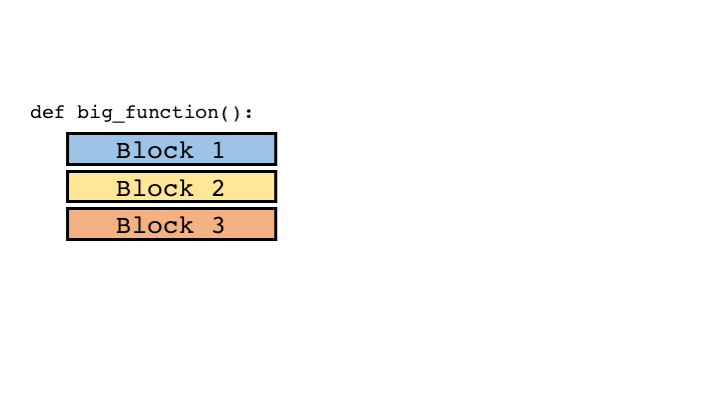
\includegraphics[width=\textwidth]{{../Figures/array_slicing/Slide36}.png}
\end{frame}

\begin{frame}[t]{Strategies for Testing: Unit Testing}
	% image
	\centering
	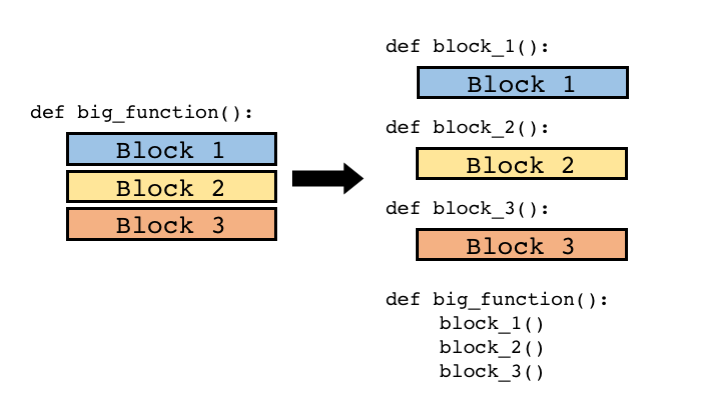
\includegraphics[width=\textwidth]{{../Figures/array_slicing/Slide37}.png}
\end{frame}

\begin{frame}[t,fragile]{unittest}
	The basic Python unit testing module is called \verb|unittest|.
	\pause
	\begin{lstlisting}
		import unittest
		
		def fun(x):
		    return x**2
			
		class FunTester(unittest.TestCase):
		    def test_case_1(self):
		        got = fun(3)
		        expected = 9
		        self.assertEqual(got,expected)
				
		if __name__=="__main__":
		    unittest.main()
	\end{lstlisting}
\end{frame}

\begin{frame}[t,fragile]{unittest}
	\begin{itemize}[<+->]
		\item \verb|unittest.main()| searches all instance of \verb|unittest.TestCase| and runs all member functions that start with ``test''.
		\item Includes many custom assertions for testing different properties of the output:
		\begin{itemize}[<+->]
			\item \verb|assertTrue(a)| - Assert that a == True.
			\item \verb|assertEqual(a,b)| - Assert that a == b.
			\item \verb|assertAlmostEqual(a,b)| - Similar to isclose.
			\item \verb|assertCountEqual| - Assert that the two sequences contain the same items, regardless of order.
			\item Many more.
		\end{itemize}
		\item Many modules extend unittest to either add features or simplify the syntax: py.test, nose, testify, etc.
	\end{itemize}
\end{frame}

\begin{frame}[t,fragile]{doctest}
	\verb|doctest| allows you to write simple test directly in a docstring.
	\pause
	\begin{lstlisting}		
		def fun(x):
			"""
			    >>> fun(3)
			    9
			"""
		    return x**2
	\end{lstlisting}
	\pause
	To run the tests call doctest on the script:
	\begin{lstlisting}		
		python -m doctest script.py
	\end{lstlisting}
\end{frame}

\end{document}
